\subsection{Coordinating Formation Control using Reinforcement Learning}

In comparison of the two methods above, A. Rawat and K. Karlapalem \cite{rawat2020multi} proposed another method using reinforcement learning to achive formation control.
The contribution of their method is stated as exploring the formation control problem through a coordination based approach using reinforcement learning, i.e. instead of following a designated leader, agents are detecting neighbor agents and trained to coordinate with them to form a specific formation.

\subsubsection{Framework}

Following the work of the authors in \cite{foerster2018counterfactual, lowe2017multi}, the paradigm of centralized training with decentralized execution is used in this work. 
They use the actor-critic architecture with a central critic as shown in Figure \ref{fig:mobilerobotrlcritic}. 

This central critic  \cite{foerster2018counterfactual} maps the true state of the system and the joint actions taken by the agents at that state to the expected future return. 
The true state of the system is defined as the pose information of all the agents with respect to the centroid of the current formation i.e. $ [x_{i}^{c},y_{i}^{c},\theta_{i}^{c}],\ \forall i \in V $ augmented with the position vector of the goal state with respect to the centroid.
A centralized experience replay is built to store the tuple of past experiences $ <s,r,s',u_{1},...,u_{|A|},o_{1},...,o_{|A|},o'_{1},...,o'_{|A|}>$, $s'$ and $o'$ are the next state of the environment and the observation of each agent in $s'$.
To speed up learning, a experience modifier similar to \cite{andrychowicz2017hindsight} is used to change the goal state to the actual state achived by the agent. 
In this case, the goal is observed with respect to different observation frames and the input to the networks is a sequence containing those goals at different time-steps.

As for actors, each agent has its history of interactions with the environment which it uses to train its policy. The decentralized execution structure is illustrated in Figure \ref{fig:multirobotfcframework}.

\begin{figure}
	\centering
	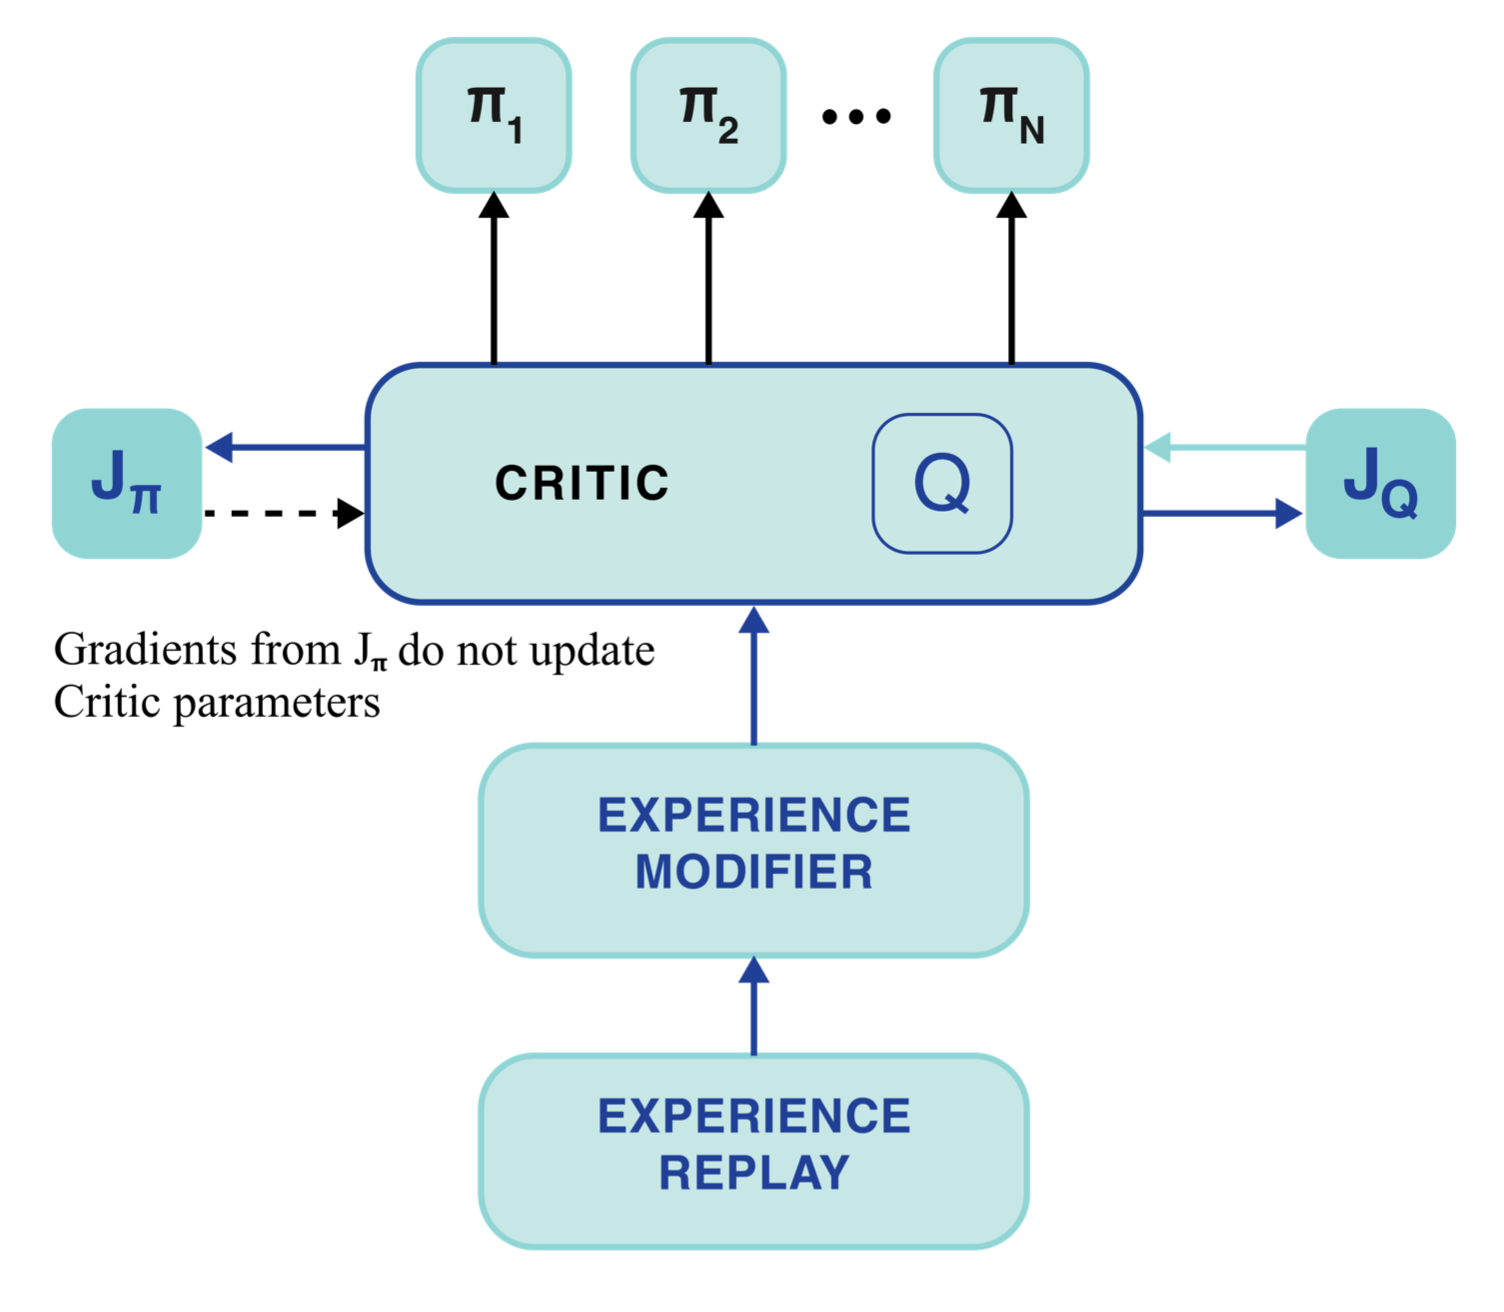
\includegraphics[width=5in]{mobilerobotrlcritic.png}
	\caption{The training involves sampling a batch of experiences, then modifying some of the experiences for positive reinforcement.}
	\label{fig:mobilerobotrlcritic} 
\end{figure}

\begin{figure}
	\centering
	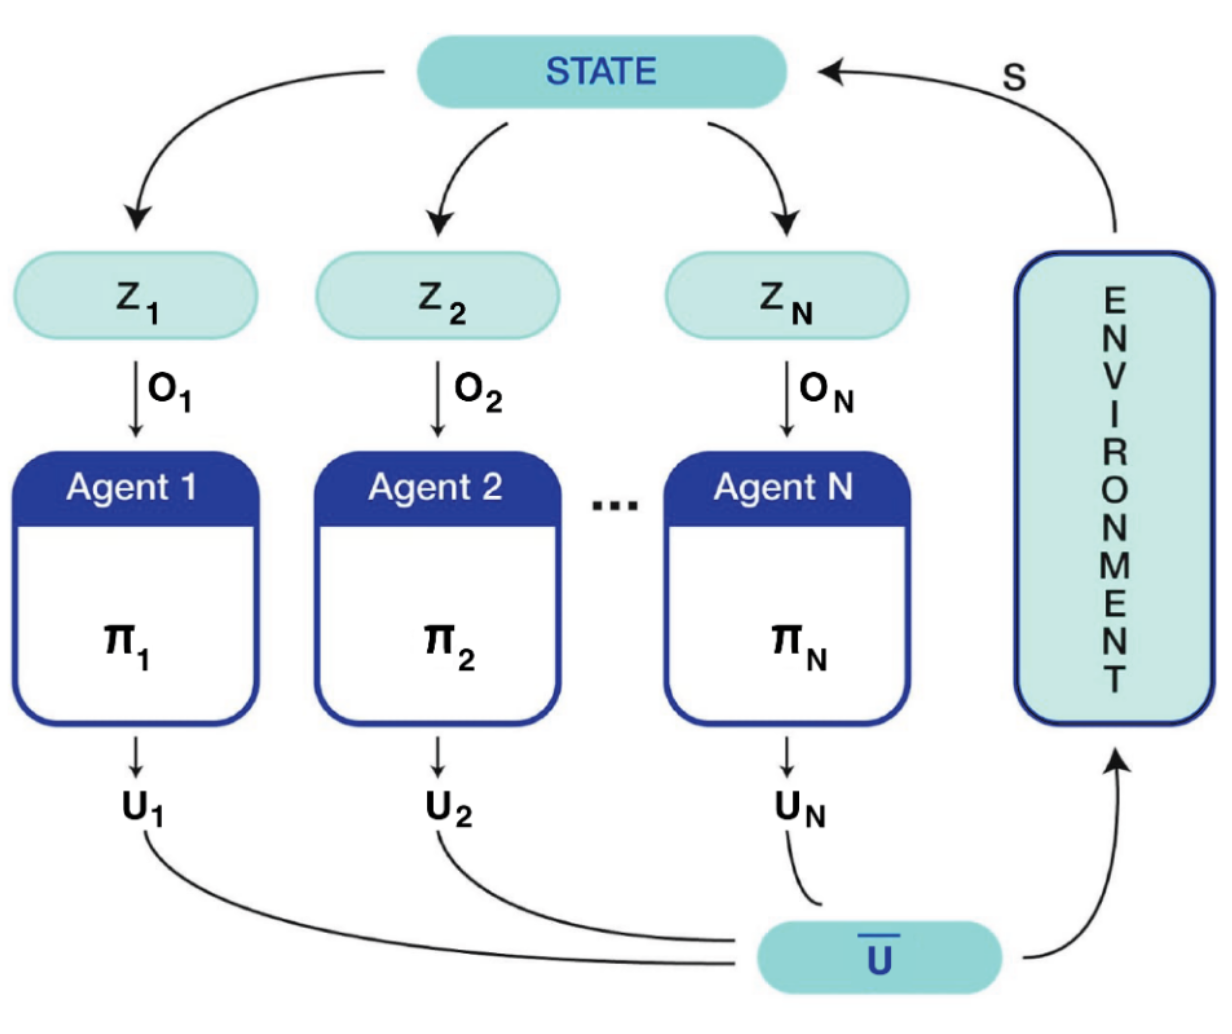
\includegraphics[width=5in]{multirobotfcframework.png}
	\caption{Interaction of agents with the environment. The state of the environment is observed through the observation function $Z_{i}$ of the agent $ i $. The agent acts according to its policy $ \pi_{i} $. The actions of all the agents $ \bar{U} $ transitions the environment to some new state.}
	\label{fig:multirobotfcframework} 
\end{figure}

\subsubsection{State Representation}

They leverage the notion of minimal rigidityand persistent graphs \cite{hendrickx2005rigidity} to define the system.
Each agent is denoted as a vortex $ v_{i} \in V $ in a graph $\mathbb{G} = (V,E) $.
There is a directed edge $e_{i,j}=(v_{i}, v_{j}) \in E$ between two agents $v_{i}, v_{j}$ if and only if agent $v_{i}$ observes agent $v_{j}$.
If each of the agents for any shape of formation observes at least two other agents then a minimally rigid graph is formed.

\subsubsection{Reinforcement}

The agents are rewarded if they are able to maintain the specific distance with the agents that they can observe. 
A reward of greater magnitude is given if the agents are able to reach the goal while maintaining said formation.
Three conditions are introduced as following, to define the reward function:

\begin{compactenum}[C1.]
	\item Formation condition: If all the agents maintain their specified edge lengths within an error of $ \epsilon_{form} $.
	\item Collision condition: This condition is met if the distance between any two agents is less than some threshold (i.e. collision), $ \epsilon_{col} $.
	\item Success condition: If formation condition is satisfied and the centroid of the formation approaches the goal within a threshold distace $ \epsilon_{goal} $.
\end{compactenum}

Then the reward function is defined as:

\begin{equation}
R(s,a,s') = \left\{
	\begin{array}{rcl}
	r_{edge}, & & {if \ only \ C1 \ is \  true}\\
	r_{collision}, & &{if\ C2\  is \  true}\\
	r_{goal}, & &{if\ C3\ is\ true}\\
	r_{penalty}, & &{otherwise}
	\end{array}
\right.
\end{equation}

\subsubsection{Experiment}

The experiment is executed in a custom environment made with the help of OpenAI gym \cite{brockman2016openai}.
The paper illustrated the error in each edge of the formation, and the distance of the centroid from the goal with respect to time for the corresponding trial, as shown in \ref{fig:mobilerobotrlresult}, also the learning curve is shown in Figure \ref{fig:mobilerobotrllearningcurve}.

\begin{figure}
	\centering
	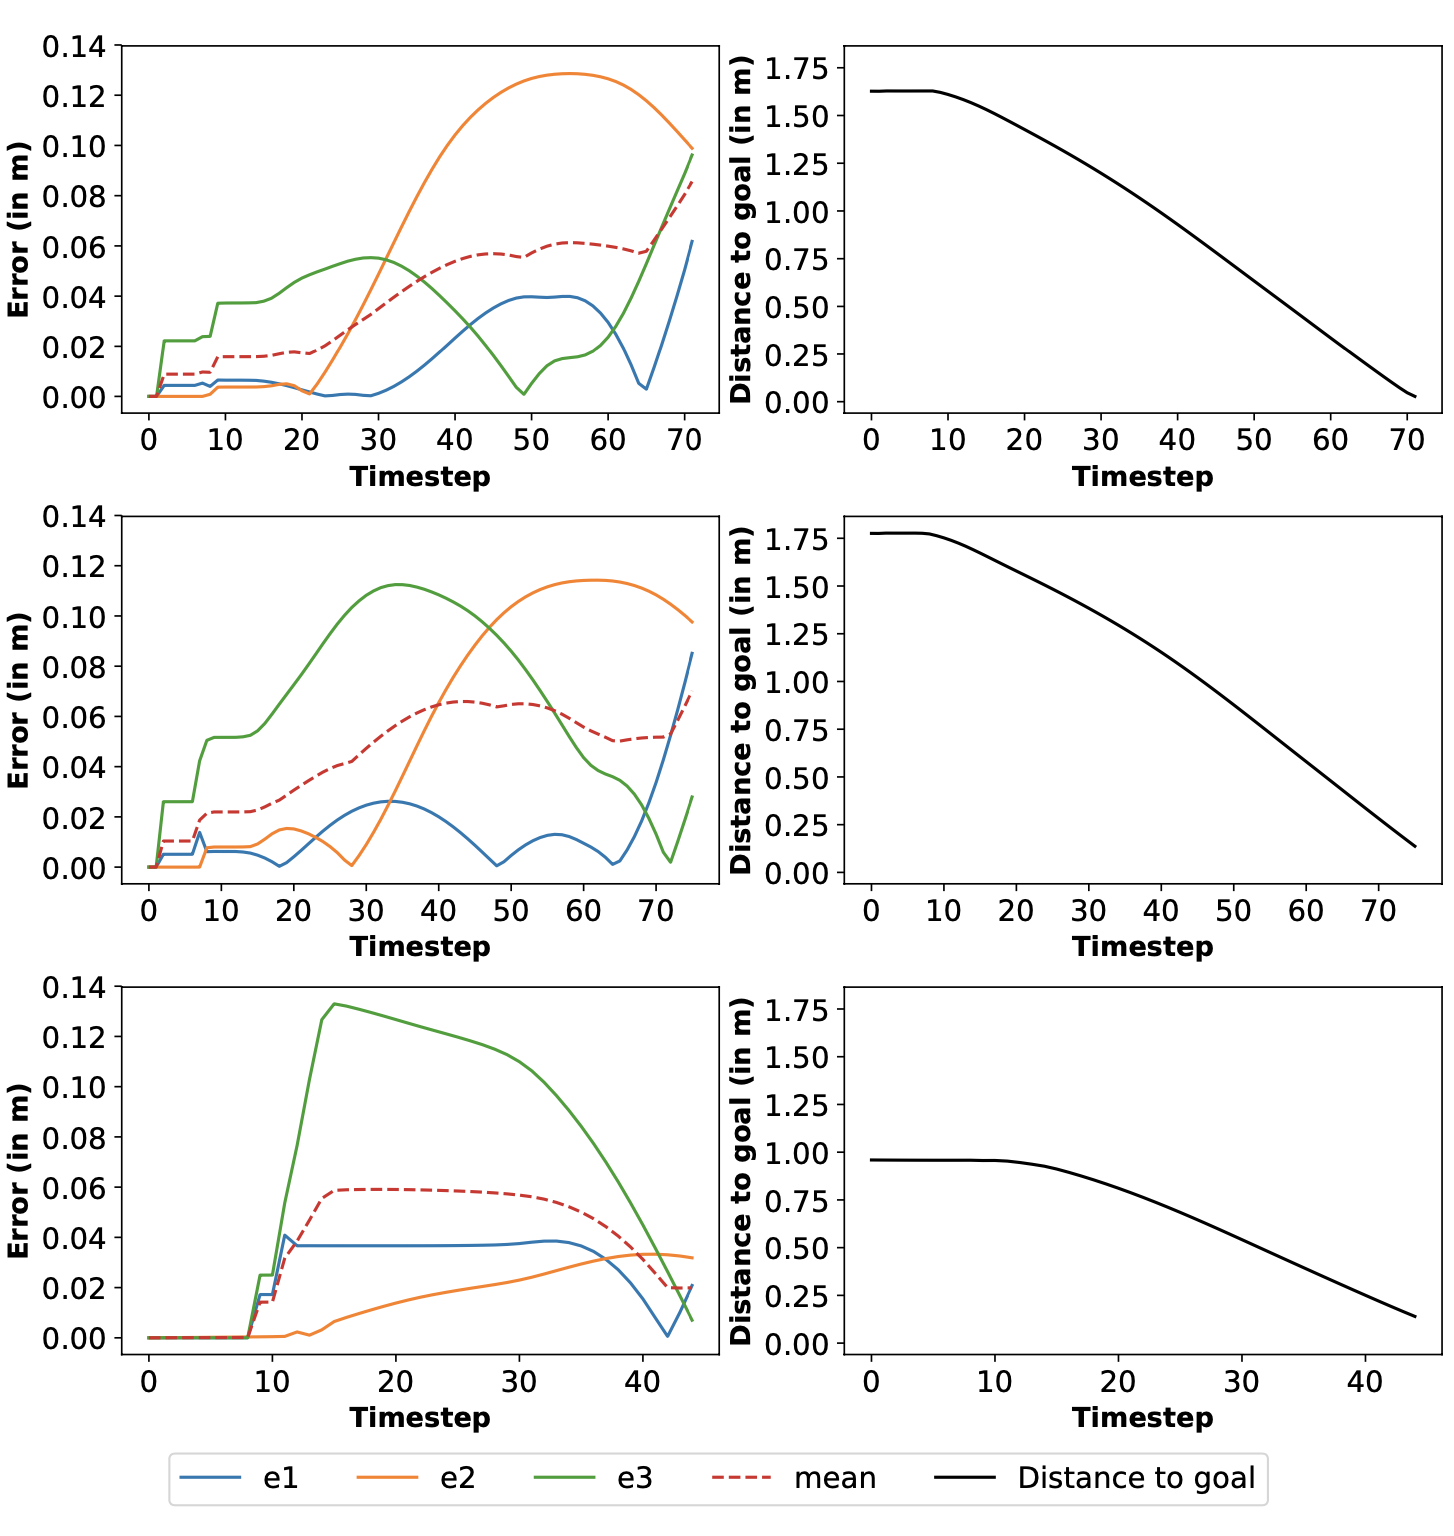
\includegraphics[width=5in]{mobilerobotrlresult.png}
	\caption{The plots on the left show the error in each edge of the formation. The plots on the right show the distance between the centroid of the formation and the goal. The edges between agents are denoted by e1, e2 and e3. The dotted red line denotes the mean error of all the edges.}
	\label{fig:mobilerobotrlresult} 
\end{figure}

\begin{figure}
	\centering
	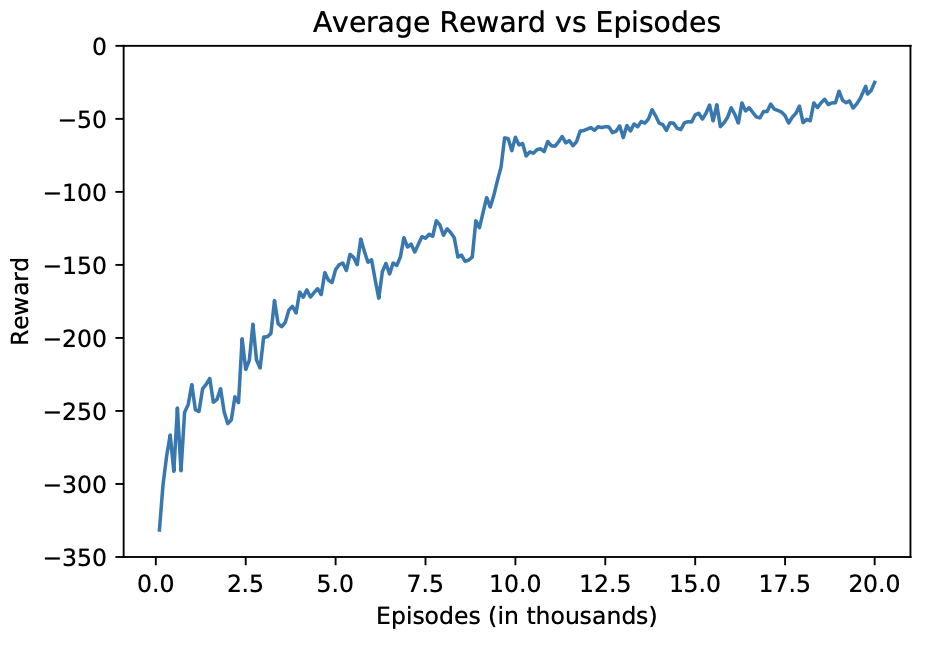
\includegraphics[width=5in]{mobilerobotrllearningcurve.png}
	\caption{Average reward per episode vs. number of training episodes.}
	\label{fig:mobilerobotrllearningcurve} 
\end{figure}

\subsubsection{Discussion}

Compared with the papers reviewed above, this method starts to use the structure of multi-agent reinforcement learning.
The combinition of a centralized critic and decentralized actors is a good application of multi-agent reinforcement learning technique.
Because it uses reinforcement learning for both target reaching and formation control, this method requires less workload to design the controller.
But also shortcomings can be concluded:

\begin{compactenum}
	\item It did not consider the problem of obstacle avoidance,
	\item This method train the deep RL network with no traditional formation control algorithm as a base, so it is suppose to require dramatically more episodes to train until at least a applicable result is attained. But the reward function definitions and full trainnig processes differ significantly between methods reviewed in this article, this possible shortcoming remains for furthur research.
\end{compactenum}
